% $Id: template.tex 11 2007-04-03 22:25:53Z jpeltier $

\documentclass{vgtc}                          % final (conference style)
%\documentclass[review]{vgtc}                 % review
%\documentclass[widereview]{vgtc}             % wide-spaced review
%\documentclass[preprint]{vgtc}               % preprint
%\documentclass[electronic]{vgtc}             % electronic version

%% Uncomment one of the lines above depending on where your paper is
%% in the conference process. ``review'' and ``widereview'' are for review
%% submission, ``preprint'' is for pre-publication, and the final version
%% doesn't use a specific qualifier. Further, ``electronic'' includes
%% hyperreferences for more convenient online viewing.

%% Please use one of the ``review'' options in combination with the
%% assigned online id (see below) ONLY if your paper uses a double blind
%% review process. Some conferences, like IEEE Vis and InfoVis, have NOT
%% in the past.

%% Figures should be in CMYK or Grey scale format, otherwise, colour 
%% shifting may occur during the printing process.

%% These few lines make a distinction between latex and pdflatex calls and they
%% bring in essential packages for graphics and font handling.
%% Note that due to the \DeclareGraphicsExtensions{} call it is no longer necessary
%% to provide the the path and extension of a graphics file:
%% \includegraphics{diamondrule} is completely sufficient.
%%
\ifpdf%                                % if we use pdflatex
  \pdfoutput=1\relax                   % create PDFs from pdfLaTeX
  \pdfcompresslevel=9                  % PDF Compression
  \pdfoptionpdfminorversion=7          % create PDF 1.7
  \ExecuteOptions{pdftex}
  \usepackage{graphicx}                % allow us to embed graphics files
  \DeclareGraphicsExtensions{.pdf,.png,.jpg,.jpeg} % for pdflatex we expect .pdf, .png, or .jpg files
\else%                                 % else we use pure latex
  \ExecuteOptions{dvips}
  \usepackage{graphicx}                % allow us to embed graphics files
  \DeclareGraphicsExtensions{.eps}     % for pure latex we expect eps files
\fi%

%% it is recomended to use ``\autoref{sec:bla}'' instead of ``Fig.~\ref{sec:bla}''
\graphicspath{{figures/}{pictures/}{images/}{./}} % where to search for the images

\usepackage{microtype}                 % use micro-typography (slightly more compact, better to read)
\PassOptionsToPackage{warn}{textcomp}  % to address font issues with \textrightarrow
\usepackage{textcomp}                  % use better special symbols
\usepackage{mathptmx}                  % use matching math font
\usepackage{times}                     % we use Times as the main font
\renewcommand*\ttdefault{txtt}         % a nicer typewriter font
\usepackage{cite}                      % needed to automatically sort the references
%\usepackage{tabu}                      % only used for the table example
%\usepackage{booktabs}                  % only used for the table example
%% We encourage the use of mathptmx for consistent usage of times font
%% throughout the proceedings. However, if you encounter conflicts
%% with other math-related packages, you may want to disable it.


%% If you are submitting a paper to a conference for review with a double
%% blind reviewing process, please replace the value ``0'' below with your
%% OnlineID. Otherwise, you may safely leave it at ``0''.
\onlineid{0}

%% declare the category of your paper, only shown in review mode
\vgtccategory{Methodological}

%% allow for this line if you want the electronic option to work properly
\vgtcinsertpkg

%% In preprint mode you may define your own headline. If not, the default IEEE copyright message will appear in preprint mode.
%\preprinttext{To appear in an IEEE VGTC sponsored conference.}

%% This adds a link to the version of the paper on IEEEXplore
%% Uncomment this line when you produce a preprint version of the article 
%% after the article receives a DOI for the paper from IEEE
%\ieeedoi{xx.xxxx/TVCG.201x.xxxxxxx}


%% Paper title.

\title{The Impacts of Data Science in Everyday Life}

%% This is how authors are specified in the conference style

%% Author and Affiliation (single author).
%%\author{Roy G. Biv\thanks{e-mail: roy.g.biv@aol.com}}
%%\affiliation{\scriptsize Allied Widgets Research}

%% Author and Affiliation (multiple authors with single affiliations).
%%\author{Roy G. Biv\thanks{e-mail: roy.g.biv@aol.com} %
%%\and Ed Grimley\thanks{e-mail:ed.grimley@aol.com} %
%%\and Martha Stewart\thanks{e-mail:martha.stewart@marthastewart.com}}
%%\affiliation{\scriptsize Martha Stewart Enterprises \\ Microsoft Research}

%% Author and Affiliation (multiple authors with multiple affiliations)
%\author{Roy G. Biv\thanks{e-mail: roy.g.biv@aol.com}\\ %
%        \scriptsize Starbucks Research %
%\and Ed Grimley\thanks{e-mail: ed.grimley@aol.com}\\ %
%     \scriptsize Grimley Widgets, Inc. }%

%% A teaser figure can be included as follows, but is not recommended since
%% the space is now taken up by a full width abstract.
%\teaser{
%  
\includegraphics[width=1.5in]{sample.eps}
%  \caption{Lookit! Lookit!}
%}

%% Abstract section.
\abstract{
The field of data science has brought about a significant transformation in decision-making processes and 
our interaction with the digital realm. This paper investigates the profound impact of data science on our everyday 
lives, delving into its core principles, diverse applications across various domains, technical obstacles encountered, 
and the emergence of novel fields of study and employment opportunities. The paper highlights the crucial stages of data 
science, which play a vital role in facilitating informed decision-making. Furthermore, it explores how data science has 
positively influenced sectors across the hole spectrum of industries while simultaneously addressing the challenges posed by 
it. Moreover, it sheds light on the birth of data analytics and artificial intelligence as exciting areas of study that are 
shaping the future job market. Lastly, ethical concerns pertaining to privacy and algorithmic bias are examined, considering 
their tangible impact on individuals' daily lives.
} % end of abstract

%% ACM Computing Classification System (CCS). 
%% See <http://www.acm.org/about/class> for details.
%% We recommend the 2012 system <http://www.acm.org/about/class/class/2012>
%% For the 2012 system use the ``\CCScatTwelve'' which command takes four arguments.
%% The 1998 system <http://www.acm.org/about/class/class/2012> is still possible
%% For the 1998 system use the ``\CCScat'' which command takes four arguments.
%% In both cases the last two arguments (1998) or last three (2012) can be empty.

\CCScatlist{
  \CCScatTwelve{data science}{big data}{data center}{data analytics};
  \CCScatTwelve{}{artificial intelligence}{data privacy}
}

%\CCScatlist{
  %\CCScat{H.5.2}{User Interfaces}{User Interfaces}{Graphical user interfaces (GUI)}{};
  %\CCScat{H.5.m}{Information Interfaces and Presentation}{Miscellaneous}{}{}
%}

%% Copyright space is enabled by default as required by guidelines.
%% It is disabled by the 'review' option or via the following command:
% \nocopyrightspace

%%%%%%%%%%%%%%%%%%%%%%%%%%%%%%%%%%%%%%%%%%%%%%%%%%%%%%%%%%%%%%%%
%%%%%%%%%%%%%%%%%%%%%% START OF THE PAPER %%%%%%%%%%%%%%%%%%%%%%
%%%%%%%%%%%%%%%%%%%%%%%%%%%%%%%%%%%%%%%%%%%%%%%%%%%%%%%%%%%%%%%%%

\begin{document}

%% The ``\maketitle'' command must be the first command after the
%% ``\begin{document}'' command. It prepares and prints the title block.

%% the only exception to this rule is the \firstsection command
\firstsection{Introduction}

\maketitle

%% \section{Introduction} %for journal use above \firstsection{..} instead
Data science has emerged as a revolutionizing field that harnesses the power of data to drive decision-making across multiple fields and industries, as 
well as transforming our interaction with the digital world. This paper seeks to explore its impact on our daily lives and address crucial issues. To begin 
the fundamentals of data science will be explained, exploring as well its process from collection to interpretation, and its importance in informed decision 
making. It will be then examined how it is being implemented in various fields, such as medicine, transportation and security, improving the quality of life 
and providing innovative solutions. Data science faces nonetheless significant technical challenges, such as handling large volumes of data and ensuring its 
quality and integrity. This paper will also inquire in some innovative approaches that are being developed to overcome these challenges and how data science 
has given rise to new branches of study and work, such as data analytics and artificial intelligence, which are shaping the employment landscape and fostering 
innovation. Finally, ethical concerns will be addressed, such as privacy and algorithmic bias, and how they affect people's daily lives.

\section{Understanding Data Science}

Data science encompasses the multidisciplinary field that combines statistical analysis, machine learning, and computational techniques and processes 
to unlock insights and knowledge from data. This involves several interconnected stages, each building upon the previous one to deliver meaningful outcomes. 
Data science is composed by the processes of data collection, cleaning, preparation, analysis, modeling, and interpretation. Let's explore each of the 
stages that compose the journey of data science:

\begin{itemize}
    \item \textbf{Data Collection:} It all begins with gathering data from various sources, such as databases, sensors, social media, or web scraping. This diverse collection 
    allows for a comprehensive understanding of the subject under study and ensures a holistic view.
    \item \textbf{Data Cleaning and Preparation:} Raw data is often messy, with inconsistencies, missing values, and errors. Data scientists employ techniques to clean 
    and preprocess the data, ensuring its quality, accuracy, and reliability for subsequent analysis.
    \item \textbf{Data Analysis:} This stage involves exploring the data using statistical methods, visualizations, and machine learning algorithms. Through data exploration, 
    patterns, correlations, and insights are discovered, providing a deeper understanding of the data and potential relationships.
    \item \textbf{Modeling and Interpretation:} In this stage, data scientists build models and algorithms that encapsulate the patterns and relationships identified during 
    analysis. These models allow for predictions, classifications, or recommendations based on the data, enabling a deeper understanding of complex phenomena.
    \item \textbf{Iterative Process:} Data science is an iterative process, meaning that each stage informs the next, and insights gained from one iteration can lead to refining 
    the entire process. Feedback loops and continuous refinement are critical to enhancing the accuracy and effectiveness of data science outcomes.
\end{itemize} 

\section{Leveraging Data Science}

In today's data-driven world, organizations across various industries have recognized the immense value of data science techniques in making informed decisions 
and gaining competitive advantages. By harnessing the power of data, these organizations can gain valuable insights and drive strategic initiatives. Data science 
enables organizations to gain a deeper understanding of their customers. Via the analysis of vast amounts of customer data, including demographics, purchase history, and 
online behavior, businesses can identify patterns and preferences. This insight allows them to personalize products, services, and marketing campaigns, resulting in 
enhanced customer satisfaction and loyalty. By analyzing operational data, such as supply chain processes, manufacturing metrics, or logistics data, businesses can 
identify bottlenecks, streamline workflows, enhance productivity, and reduce costs. Through data science, organizations can leverage historical data to predict future 
trends and behaviors. Companies employing techniques like regression analysis, time series forecasting, and predictive modeling, businesses can anticipate market demands, 
customer preferences, and potential risks. This foresight enables proactive decision-making and strategic planning. Product development and quality improvement is another 
area in which through analysis of customer feedback, user behavior data, and product usage metrics, businesses can uncover insights to enhance product features, usability, 
and overall user experience. These data-driven improvements help organizations stay ahead of the competition but also benefits the customers who get better value for their money.\newline

However, the advances in this field not only benefit large companies, but also ordinary people all around the world in a wide variety of areas. Many significant advancements in 
healthcare have been achieved by leveraging large datasets and developing algorithms that help medical professionals make more accurate diagnoses, predict disease outcomes, and 
personalize treatment plans. Machine learning algorithms, which are another result of advances in data science, can analyze medical records, genetic data, and clinical research 
to improve patient care and outcomes. Dr. Najat Khan Chief Data Science Officer and Global Head at the Janssen Pharmaceutical Companies of Johnson \& Johnson talked in an interview 
about how parmaceuticals are helping patients with this new tecnologies: "Imagine that a patient has a specific mutation of cancer for which there is a targeted therapy. However, currently, 
these mutations are not picked up in a routine way because they are new and therefore are not sequenced on a regular basis. But every patient gets their tumor biopsied, so what we have 
done is used data science to digitize those biopsy slides, and then we use machine learning model to predict what mutation a patient might have just from those images. The impact of 
that is to find diseases earlier in patients who could benefit from a targeted therapy and may otherwise have been missed."\cite{Robinson:2022} The financial industry has too  been 
revolutionized , enabling faster and more accurate risk assessments, fraud detection, and personalized financial advice. Via the analysis of transaction data and patterns, banks can 
detect suspicious activities and protect customers' financial assets. Data science techniques are also vital in cybersecurity to detect and prevent threats. By assessing network logs, 
user behavior patterns, and anomaly detection algorithms, governments, companies and people can identify potential security breaches and fraud attempts. This proactive approach strengthens 
cybersecurity measures and safeguards sensitive data from unauthorized access.

\section{Technical challenges of Data Science}

Looking back to the processes of data science it is possible to realize that as the size of the data to be used increases, multiple challenges arise.
Analyzing massive datasets, commonly known as big data, presents a unique set of challenges due to the volume, velocity, variety, and veracity of 
the data. While big data offers immense potential for generating valuable insights, it also requires specialized approaches and technologies to 
overcome these challenges. First of all to generate big amounts of data, multiple types of hardware are required such as sensors, microprocessors and computers
.Incrementing the amount of collection devices requires some considerable commitment and big investments that can limit the hability of most people and small 
companies to obtain the desired or needed results. After collecting the information, it is necessary to ensure the quality of the data used for the analysis. Data 
sets may contain errors, outliers or incomplete information, which can affect the accuracy of the models and the results obtained. To address this problem, multiple 
specialists are needed to select the data to be used and to filter out what is not relevant or may have a negative effects and to further streamline processes and eliminate 
repetitive tasks, data cleaning and preprocessing techniques are also being developed, including error detection and correction, imputation of missing values and 
identification of outliers.\newline

Big data often exceeds the storage and computational capabilities of traditional systems. Managing and storing massive volumes of data requires scalable infrastructure, 
such as distributed file systems and cloud-based solutions. Similarly, processing and analyzing such vast amounts of data necessitate distributed computing 
frameworks,\footnote{A distributed computing framework refers to a software framework that allows the coordination and utilization of multiple computers (also known 
as nodes) connected over a network to work collectively.} like Hadoop or Apache Spark that can parallelize computations across clusters of machines. In addition to all these 
hardware and trained personnel requirements, it is necessary to build infrastructure to house all these systems, also known as data centers. Construction requirements include 
choosing a suitable site that meets security standards, access to reliable electrical power services, access to high-speed communication networks and scalability for future expansion. 
It is also necessary to design a robust physical infrastructure that includes redundant power supply systems, efficient cooling systems for the computers that run day and night, and 
security systems to protect the equipment and stored data. According to an analysis by the UK-founded commercial real estate services company Lang LaSalle Incorporated "the 
average-powered base building (defined here as foundation, four walls and roof along with a transformer and common areas for security, loading dock, restrooms, corridors, etc…) of a 
data center facility typically ranges from 125 US-dollars per square foot to upwards of 200 per square foot."\cite{Hawkins:2022} On top of these costs, getting a data center ready to function 
with all IT capabilities can cost between "280 US-dollars per square foot and 350 per square foot."\cite{Hawkins:2022} These costs can, of course, be much higher depending on the location 
of construction as well as power and availability requirements. To provide an example, when Facebook started constructing the Prineville Data Center in Oregon USA back in 2009 the 
company invested more than a billion US-dollars to construct the 1.25 million-square-foot facility.

Data science involves extracting meaningful information from large volumes of data. Nevertheless, proper interpretation of the results can be challenging. Machine learning 
models and analysis techniques can generate complex results that require deep and expert understanding for interpretation. This is why multiple companies and governments are 
constantly looking for educated and skilled workers to help them get the right results. Another way data scientists are addressing this challenge is through the development of 
visualization methods and model explainability techniques that help understand and communicate results more effectively.

\section{The emergence of new branches of study and work}

The rapid rise of data science has led to the emergence of new fields of study and has created exciting opportunities in the job market. As 
companies increasingly recognize the value of data-driven decision making, the demand for qualified data science professionals continues to grow.
 
\subsection{Studies on data science}


\subsection{labor demand in data science}

\begin{figure}[tb]
  \centering % avoid the use of \begin{center}...\end{center} and use \centering instead (more compact)
  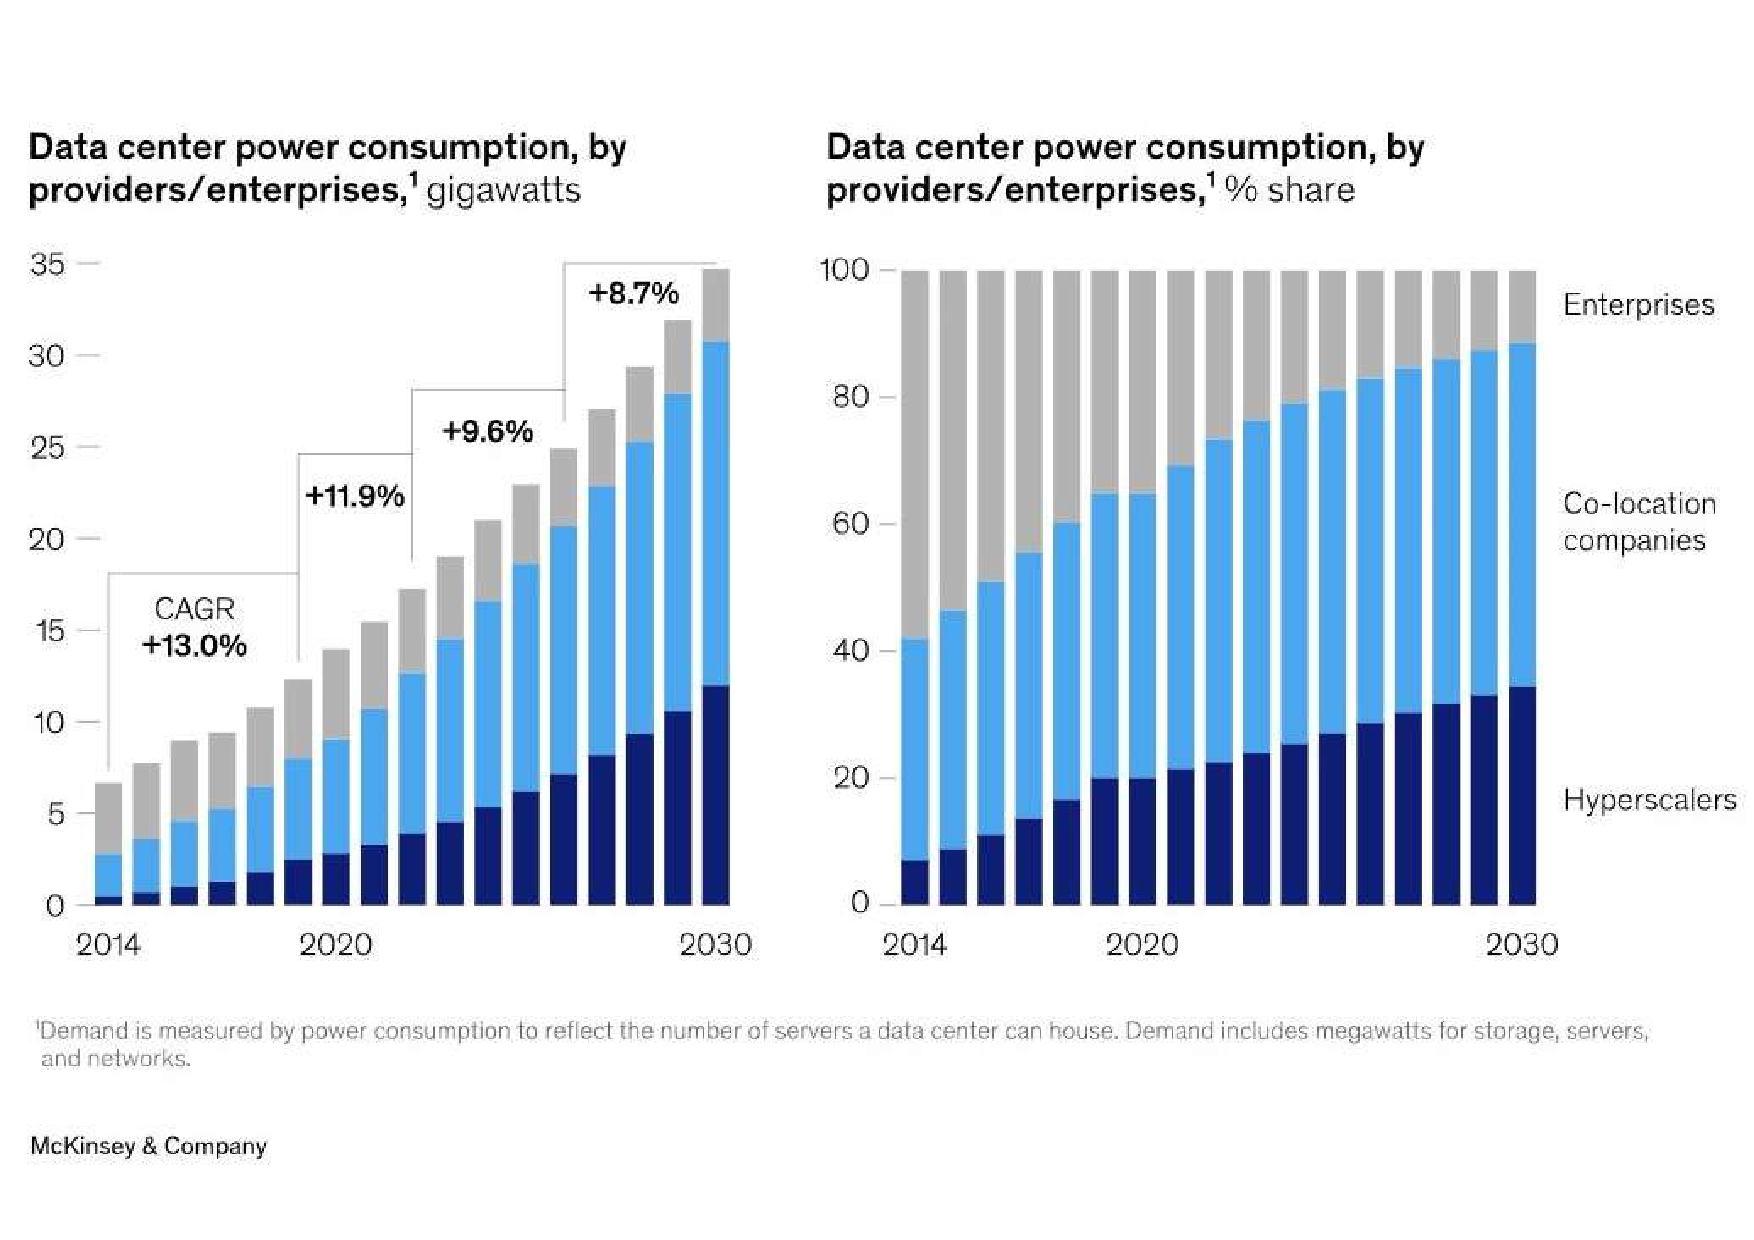
\includegraphics[width=\columnwidth]{datacenter_demand}
  \caption{A visualization of the 2014--2030 forecast data of US data center demand. The image is from \cite{Bangalore:2023} and is in the public domain.}
  \label{fig:sample}
 \end{figure}

\section{Artificial intelligence}


\section{Ethical Issues}

vel eum iriure dolor in hendrerit
in vulputate velit esse molestie consequat,\footnote{Footnotes
appear at the bottom of the column.} vel illum dolore eu
feugiat nulla facilisis at vero eros et accumsan et iusto odio
dignissim qui blandit praesent luptatum zzril delenit augue duis
dolore te feugait nulla facilisi. Lorem ipsum dolor sit amet,
consectetuer adipiscing elit, sed diam nonummy nibh euismod tincidunt
ut laoreet dolore magna aliquam erat volutpat.

\section{Conclusion}

Lorem ipsum dolor sit amet, consetetur sadipscing elitr, sed diam
nonumy eirmod tempor invidunt ut labore et dolore magna aliquyam erat,
sed diam voluptua. At vero eos et accusam et justo duo dolores et ea
rebum. Stet clita kasd gubergren, no sea takimata sanctus est Lorem
ipsum dolor sit amet. Lorem ipsum dolor sit amet, consetetur
sadipscing elitr, sed diam nonumy eirmod tempor invidunt ut labore et
dolore magna aliquyam erat, sed diam voluptua. At vero eos et accusam
et justo duo dolores et ea rebum. Stet clita kasd gubergren, no sea
takimata sanctus est Lorem ipsum dolor sit amet. Lorem ipsum dolor sit
amet, consetetur sadipscing elitr, sed diam nonumy eirmod tempor
invidunt ut labore et dolore magna aliquyam erat, sed diam
voluptua. At vero eos et accusam et justo duo dolores et ea
rebum.


%% if specified like this the section will be committed in review mode
\acknowledgments{
The authors wish to thank A, B, and C. This work was supported in part by
a grant from XYZ.}

%\bibliographystyle{abbrv}
\bibliographystyle{abbrv-doi}
%\bibliographystyle{abbrv-doi-narrow}
%\bibliographystyle{abbrv-doi-hyperref}
%\bibliographystyle{abbrv-doi-hyperref-narrow}

\bibliography{template}
\end{document}
